\documentclass[14pt]{article}
\usepackage[russian]{babel}
\usepackage{graphics}
\usepackage{colortbl}
\usepackage{amsmath,amsfonts,amssymb}
\usepackage[unicode,pdftex]{hyperref}
\usepackage{geometry}
\linespread{1}
\usepackage[unicode, pdftex]{hyperref}
\geometry{
	a4paper,
	top=13.8mm,
	right=12mm,
	bottom=4.9mm,
	left=13.1mm
}
\begin{document}
	\begin{center}
		\small \textbf{Санкт-Петербургский национальный} \\\textbf{исследовательский университет} \\
		\textbf{информационных технологий, механики и оптики} \\ 
		\textbf{УЧЕБНЫЙ ЦЕНТР ОБЩЕЙ ФИЗИКИ ФТФ} \\
		
\includegraphics{ItmoLogo.png}
	\end{center} 
	\noindent\rule{18.5cm}{3pt} \\ \\
	\large Группа\noindent\rule{7cm}{0.5pt} К работе допущен \noindent\rule{6.5cm}{0.5pt} \\ \\ \\
	Студен \noindent\rule{7cm}{0.5pt} Работа выполнена \noindent\rule{6.5cm}{0.5pt} \\
	\begin{center}
		Преподаватель \noindent\rule{4cm}{0.5pt} Отчет принят \noindent\rule{6.5cm}{0.5pt}
	\end{center} 
	\begin{center}
		\Huge \textbf{Рабочий протокол и отсчет} \\\textbf{по лабораторной работе №1} 
	\end{center}
	\noindent\rule{18.5cm}{2pt}
	\begin{center}
		\textbf{Исследование распределения случайной величины}
	\end{center}
	\noindent\rule{18.5cm}{2pt} \\ \\
	\textbf{1. Цель работы.} 
	\par 1) Провести измерения конкретного интервала времени 
	\par 2) Построить гистограмму результатов измерения 
	\par 3) Вычислить среднее значение и дисперсию 
	\par 4) Сравнить гистограмму с графиком функции Гаусса с таким же распределением средним значением и дисперсией \\
	\textbf{2. Задачи, решаемые при выполнении работы.} 
	\par 1) Провести 50 измерений, устанавливая промежуток времени в 7 секунд. Результаты вносить в таблицу;
	\par 2) Построить гистограмму по алгоритму, прописанному в выполнении работы;
	\par 3) По данным таблицы вычислить выборное значение среднего $\langle t \rangle N$ и выборочное среднеквадратичное отклонение $\sigma N$;
	\par 4) Записать результаты в таблицу;
	\par 5) По формуле вычислить максимальное значение плотности распределения $\rho_max$ соответствующее $t=\langle t \rangle$, занести его в таблицу;
	\par 6) Найти значение $t$, соответствующие серединам выбранных ранее интервалов, занести их в столбец новой таблицы номер 2. Для этих значений, используя параметры $\langle t \rangle N$ и $\sigma N$ в качестве $\langle t \rangle$ и $\sigma$, вычислить значение плотности распределения $\rho (t)$, занести их в новую таблицу номер 2. Нанести все расчетные точки на график, на котором изображена гистограмма и провести через них плавную кривую;  
	\par 7) Проверить, насколько точно выполняется в наших опытах соотношение между вероятностями и долями $\frac{\Delta N_{\sigma}}{N},\frac{\Delta N_{2\sigma}}{N},\frac{\Delta N_{3\sigma}}{N}$. Для этого вычислить границы интервалов для найденных нами значений $\langle t \rangle N$ и $\sigma N$, занести их в таблицу номер 3; 
	\par 8) По данным первой таблицы подсчитать и занести в таблицу номер 3 количество $\Delta N$ измерений, попадающих в каждый их этих интервалов, и отношение $\frac{\Delta N}{N}$ этого количества к общему числу измерений. Сравнить их с соответствующими нормальному распределению значениями $P$ вероятности; 
	\par 9) Рассчитать среднеквадратичное отклонение среднего значения 
	\par 10) Найди табличное значение коэффициента Стьюдента $t_{\alpha,N}$ для доверительной вероятности $\alpha=0,95$. Записать доверительный интервал для измеряемого в работе промежутка времени \\
	\textbf{3. Объект исследования.} 
	\par Промежуток времени длительностью в 7 секунд \\
	\textbf{4. Метод Экспериментального исследования} 
	\par Стрелочным секундомером задается интервал времени, который многократно измеряется цифровым секундомером \\
	\textbf{5. Рабочие формулы и исходные данные} \\
	\begin{tabular}{| c | l |}
		\hline
		$\langle t \rangle N=\frac{1}{N}(t_1+t_2+\dots+t_N)=\frac{1}{N}\overset{N}{\underset{i=1}{\Sigma}}t_i$ & $\langle t \rangle N$ - выборочное значение \\ \hline 
		$\rho(t)=\frac{1}{\sigma \sqrt{2 \pi}}\exp \left(-\frac{(t-\langle t \rangle )^2}{2\sigma^2}\right)$ & $\rho(t)$ - плотность вероятности или закон распределения\\ 
		& исследуемой величины  \\
		\hline
		$\sigma_N = \sqrt{\frac{1}{N-1}\overset{N}{\underset{i=1}{\Sigma}}(t_i-\langle t \rangle_N)^2}$ & $\sigma N$ - выборочное среднеквадратичное отклонение \\
		\hline 
		$\rho_{\max}=\frac{1}{\sigma\sqrt{2\pi}}$ & $\rho_{\max}$ - максимальная высота гистограммы \\
		\hline 
		$[\langle t \rangle_N - \sigma_N ,\langle t \rangle_N + \sigma_N]$, & $P$ - вероятность попадания результата каждого \\
		$[\langle t \rangle_N - 2 \sigma_N,\langle t \rangle N + 2\sigma_N],$ & измерения в интервал $[t_1,t_2]$ \\
		$[\langle t \rangle_N - 3 \sigma_N, \langle t \rangle_N + 3 \sigma_N]$ & \\
		\hline
		$\sigma_{\langle t \rangle }=\sqrt{\frac{1}{N(N-1)}\overset{N}{\underset{i=1}{\Sigma}}(t_i-\langle t \rangle_N)^2}$ & $\sigma$ - среднеквадратичное отклонение среднего значения \\
		\hline 
		& $t_{\alpha,N}$ - коэффициент Стьюдента,\\$\Delta t = t_{\alpha,N} \cdot \sigma_{\langle t \rangle},\; \alpha = 0,95$  & \\
		&  $\alpha$ - доверительная вероятность \\
		\hline
	\end{tabular} \\ \\ \\
	\textbf{6. Измерительные приборы} \\ \\
	\begin{tabular}{|c|c|c|c|c|}
		\hline
		\textit{№ п/п} & \textit{Наименование} & \textit{Тип прибора} & \textit{Используемый диапазон} & \textit{Погрешность прибора} \\
		\hline
		\textit{1} & Секундомер & Механический & 7 секунд & $\pm 0.1$с \\
		\hline 
		\textit{2} & Секундомер & Электронный & 7 секунд & $\pm (9.6 \cdot 10^{-6}+0.01)$с \\
		\hline
	\end{tabular} \\ \\ \\
	\textbf{7. Результаты измерений и их обработки} \\ \\
	\begin{tabular}{|p{1cm}|p{5cm}|p{5cm}|p{5cm}|}
		\hline
		№ & $t_i$, с & $t_i -\langle t \rangle_N$,с & $(t_i-\langle t \rangle_N)^2$, c$^2$ \\
\hline
1 & 6.78 & 0.203 & 0.0412 \\
\hline
2 & 7.1 & -0.117 & 0.0137 \\
\hline
3 & 7.04 & -0.057 & 0.0032 \\
\hline
4 & 6.95 & 0.033 & 0.0011 \\
\hline
5 & 6.61 & 0.373 & 0.1391 \\
\hline
6 & 7.06 & -0.077 & 0.0059 \\
\hline
7 & 6.94 & 0.043 & 0.0018 \\
\hline
8 & 7.0 & -0.017 & 0.0003 \\
\hline
9 & 6.94 & 0.043 & 0.0018 \\
\hline
10 & 7.0 & -0.017 & 0.0003 \\
\hline
11 & 7.03 & -0.047 & 0.0022 \\
\hline
12 & 7.13 & -0.147 & 0.0216 \\
\hline
13 & 6.78 & 0.203 & 0.0412 \\
\hline
14 & 7.02 & -0.037 & 0.0014 \\
\hline
15 & 6.99 & -0.007 & 0.0 \\
\hline
16 & 6.82 & 0.163 & 0.0266 \\
\hline
17 & 6.82 & 0.163 & 0.0266 \\
\hline
18 & 7.03 & -0.047 & 0.0022 \\
\hline
19 & 7.13 & -0.147 & 0.0216 \\
\hline
20 & 7.02 & -0.037 & 0.0014 \\
\hline
21 & 6.97 & 0.013 & 0.0002 \\
\hline
22 & 7.21 & -0.227 & 0.0515 \\
\hline
23 & 7.02 & -0.037 & 0.0014 \\
\hline
24 & 6.93 & 0.053 & 0.0028 \\
\hline
25 & 7.0 & -0.017 & 0.0003 \\
\hline
26 & 6.9 & 0.083 & 0.0069 \\
\hline
27 & 6.82 & 0.163 & 0.0266 \\
\hline
28 & 7.1 & -0.117 & 0.0137 \\
\hline
29 & 6.94 & 0.043 & 0.0018 \\
\hline
30 & 6.79 & 0.193 & 0.0372 \\
\hline
31 & 7.13 & -0.147 & 0.0216 \\
\hline
32 & 7.0 & -0.017 & 0.0003 \\
\hline
33 & 6.94 & 0.043 & 0.0018 \\
\hline
34 & 6.99 & -0.007 & 0.0 \\
\hline
35 & 7.13 & -0.147 & 0.0216 \\
\hline
36 & 7.08 & -0.097 & 0.0094 \\
\hline
37 & 6.98 & 0.003 & 0.0 \\
\hline
38 & 6.95 & 0.033 & 0.0011 \\
\hline
39 & 7.14 & -0.157 & 0.0246 \\
\hline
40 & 6.87 & 0.113 & 0.0128 \\
\hline
41 & 7.12 & -0.137 & 0.0188 \\
\hline
42 & 7.0 & -0.017 & 0.0003 \\
\hline
43 & 6.94 & 0.043 & 0.0018 \\
\hline
44 & 7.1 & -0.117 & 0.0137 \\
\hline
45 & 7.0 & -0.017 & 0.0003 \\
\hline
46 & 7.0 & -0.017 & 0.0003 \\
\hline
47 & 6.97 & 0.013 & 0.0002 \\
\hline
48 & 6.98 & 0.003 & 0.0 \\
\hline
49 & 7.01 & -0.027 & 0.0007 \\
\hline
50 & 6.95 & 0.033 & 0.0011 \\ 
		\hline
		& $\langle t \rangle N$ = 6.983 & $\underset{i=1}{\overset{N}{\Sigma}}(t_i-\langle t \rangle_N)=-2.5e^{-14}$ & $\sigma _N= 0.0128 $ \\
		& & & $\rho_{\max}=31.2146$ \\
		\hline
	\end{tabular} \\ \\ \\	
	\textbf{8. Расчет результатов косвенных измерений.} \\ \\ 
	\begin{tabular}{|p{3cm}|p{3cm}|p{3cm}|p{3cm}|p{3cm}|}
		\hline Границы интервалов, с & $\Delta N$ & $\frac{\Delta N}{N \Delta t},$с$^{-1}$ & $t$, c & $\rho$, c$^{-1}$ \\
		\hline
		$[ 6.61 ; 6.6957 ]$ & 1 & 0.2333 & 6.6529 & 0.0153 \\
		\hline
		$[ 6.6957 ; 6.7814 ]$ & 2 & 0.4667 & 6.7386 & 0.1398 \\
		\hline
		$[ 6.7814 ; 6.8671 ]$ & 4 & 0.9333 & 6.8243 & 0.7199 \\
		\hline
		$[ 6.8671 ; 6.9529 ]$ & 11 & 2.5667 & 6.91 & 2.0873 \\
		\hline
		$[ 6.9529 ; 7.0386 ]$ & 19 & 4.4333 & 6.9957 & 3.4056 \\
		\hline
		$[ 7.0386 ; 7.1243 ]$ & 7 & 1.6333 & 7.0814 & 3.1273 \\
		\hline
		$[ 7.1243 ; 7.21 ]$ & 6 & 1.4 & 7.1671 & 1.6161 \\
		\hline
	\end{tabular} \\ \\
	\textbf{9. Расчет погрешностей измерений} \\ \\ 
	\begin{tabular}{|p{3cm}|p{3cm}|p{3cm}|p{3cm}|p{3cm}|}		
		\hline
		& Интервал, с &  & & \\
		& От и До &$\Delta N$ & $\frac{\Delta N}{N}$ & $P$ \\
		\hline 
		$\langle t \rangle_N \pm \sigma_N$ & 6.9958, 6.9702& 4 & 0.08 & 0.683 \\
		\hline 
		$\langle t \rangle_N \pm 2\sigma_N$ & 7.0086, 6.9574& 13 & 0.26 & 0.954\\
		\hline 
		$\langle t \rangle_N \pm 3\sigma_N$ & 7.0213, 6.9491& 20 & 0.4 & 0.997 \\
		\hline
	\end{tabular} \\ \\ \\
	\textbf{10. Графики.} \\ \\
	\begin{center}
	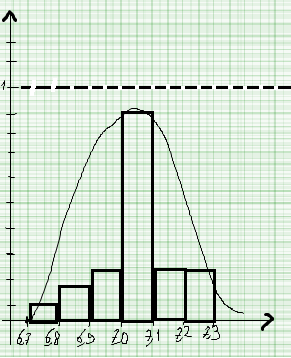
\includegraphics{gistogramma.png} 
	\end{center}
	\textbf{11. Выводы и анализ результатов работы.} 
	\par В данном эксперименте я не могу гарантировать, что все действия были совершены идеально, ведь человеческие руки не в состоянии точно нажимать на кнопку "стоп" и "старт" и из-за этого появлялись погрешности и из-за этого таблица имела отличия с нормальным распределением Гаусса. Также на результат повлияла малое число измерений. При большим числе (к примеру 1000) результат мог бы быть более точным. Однако, можно заметить, что они имеют схожую динамику. \\ \\
	\textbf{12. Дополнительные задания} 
	\\ \\
	\textbf{13. Выполнение дополнительных заданий}
	\\ \\
	\textbf{14.	Замечания преподавателя (исправления, вызванные замечаниями преподавателя, также помещают в этот пункт.}
\end{document}
